\section{The climate crisis: addressing a contemporary issue}

Traditionally, museums have been a window to the past, "a place where the past lives”. My research aim to provide insight of how museums can play a central role in addressing contemporary issues, like the climate crisis.

The public discussion on the climate crisis is what I refer to as the climate debate. As a museum discourse, the climate debate represents and has some characteristics that open for new ways of thinking on why the museum space is an ideal space for exhibiting the discourse, on new ways of designing for contemporary issues, engaging a broad audience, and using embedded interactivity to design meaningful museum experiences.

\begin{figure}[h]
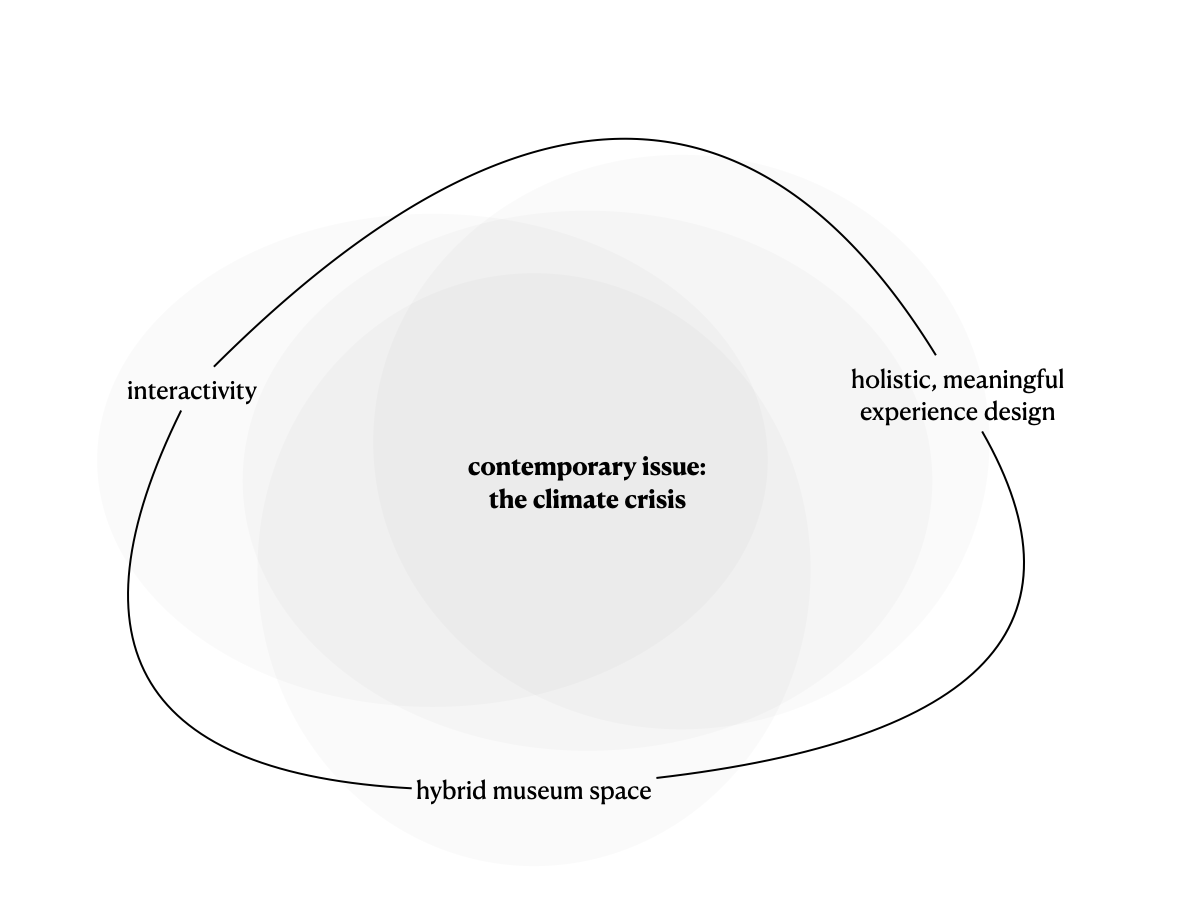
\includegraphics[width=10cm]{pictures/problem_sphere.png}
\caption{My representation of sustainability issues in museums}
\centering 
\end{figure}

\section{Museums addressing climate change and sustainability}
In a commentary by Richard J. Hebda, it is looked into the Royal British Columbia Museum (RBCM)’s voyage into the issue of climate change as an example of how museums can play a central role in addressing contemporary issues. Traditionally, museums have been a window to the past, "a place where the past lives" \autocite[p. 1]{hebda_article}.  Traditionally, museums trot out historical artifacts, old plant and animal specimens, and host great exhibits on famous people, events and cultures \autocite[p.1]{hebda_article}.
\par
A lot of the issues and societal attitudes that are addressed in the commentary are still relevant today. Traditionally in museums, human and natural history is seen as two solitudes that have been exhibited separately. A key appeal for the RBCM, a typical natural history museum to do a climate change exhibit, was to pursue the opportunity to link and integrate the two solitudes in a compelling and relevant manner \autocite[p. 2]{hebda_article}. They justify that the integration is necessary because the challenge is central in the sustainability debate because the progressive separation of human and natural science is at the core of the problem facing society today \autocite[p.2]{hebda_article}.

In 2007 when the RBCM decided to make the climate change exhibition, the question of climate change was still a controversial issue \autocite[p.2]{hebda_article}. Addressing the increasing evidence and knowledge in terms of climate change and how it affects and is affected by humans, nearly all reputable scientists felt that change was under way and action was needed \autocite[p.2]{hebda_article}. The political and public atmosphere was foggy, as people did not know whom to believe, what information was science-based rather than rhetoric, and where real uncertainty lay \autocite[p.2]{hebda_article}. The RBCM saw a clear opportunity to dispel the fog and to enlighten their audiences \autocite[p.2]{hebda_article}.

To begin with, the museum simply wanted to update the entrance to the natural gallery where climate was briefly explored, but saw the opportunity to create an exhibit where (... this, this and this is adressed). And then write a summary of the case and results of the article.:
- (this was perhaps) a reflection of society’s general lack of recognition of climate’s central role in shaping the world and our lives.
- The museum also struggled with the need to be more socially relevant.


\subsection{Sustainability as a contemporary issue}



 
\subsection{Notes}
Hvordar forstår jeg bærekraft, og hvorfor mener jeg det er viktig?
Hvordan snakker andre om det, og hva må jeg få sagt til leseren om bærekraft?
Hvordan “angriper” jeg bærekraft temaet inn i denne oppgaven?

Hva slags utfordringer er det for museer som tematisk jobber med, /formidler, bærekraft?

(Prosess) Hvordan min prosess er farget av det jeg er opptatt av

Rapportering nytt kapittel

Hvordan er prosessen min koblet til teorien?



\subsection{Sustainability as a subject for cultural analysis in museums}
Mieke Bal is a dutch cultural theorist, video artist and Professor in Literary Theory at the University of Amsterdam, with academic interest and background in humanities, media and culture studies. From her writings on the discourse of the museum, she discusses what differentiates the “new” museology from the “old”, and presents the museum as a discourse and the exhibition as an utterance within that discourse. Bringing this discursive perspective to the museum deprives the museal practise of its innocence, and provides it with the accountability it and its users are entitled to (Thi, p. 214). Part of her argument is that politics come straight out of, or more precisely are bound up with, the museal discourse (Thi, p. 214), and proposes a threefold direction to museology researchers. First she suggest to systematically analyse the narrative-rhetorical structure of the specific museum, in order to refine the categories and deepen insight into their effects. Secondly she suggest to look at the connection between the museal discourse and the institutions foundation and history, and thirdly she see the need to do self-critical analysis of the museal discourse as a consequence of the nature of discourse.

With my background and scope of thesis it is both irrelevant and I am by no means capable to do a discursive analysis in the way Mieke Bal proposes. I do however find aspects of Bal’s discursive perspective relevant, like her proposal of how one can do a narrative-rhetorical systematic analysis of a specific museum. She provides a set of new terms and vocabulary so that I better can “read”, describe, understand and do research on a specific museum and/ or specific installation. I find this perspective along with the extended vocabulary it provides useful so that I better can identify meaningful relations between user activity at installations/ artefacts and the museum experience.